\section{Buscas}
\subsection{Importância}
\begin{frame}{Buscas - Importância}
	\begin{itemize}
		\item Certeza de encontrar todas as incidências
		\item Ficam visualmente destacadas (com :set hlsearch)
		\item Testar substituições
		\item Verificar a ortografia atrás de erros de digitação
		\item Encontrar variáveis ou funções não utilizadas, só declaradas
		\item Encontrar rapidamente algum termo
		\item Verificar a existência de algum termo
	\end{itemize}
\end{frame}

\subsection{Buscando com eficiência}
\begin{frame}{Buscando com eficiência}
	\begin{description}
		\item[/termo] Busca pela incidência de \textit{termo} nos arquivos abertos
		\item[:vimgrep] Abre os arquivos com a incidência do termo na Quickfix List
		\item[:vimgrepadd] Adiciona novos arquivos e incidências a Quickfix List
		\item[:grep] Executa um comando externo e abre os arquivos resultados (set grepprg)
		\item[:!grep] Apenas mostra o output do comando externo
	\end{description}
\end{frame}
\begin{frame}{/termo}
	\begin{block}{Exemplos}
	\begin{itemize}
		\item /texto
		\item /\textbackslash\textless{}casa\textbackslash\textless
		\item /\$var
		\item /public void static Main(String\textbackslash[\textbackslash] args)
		\item /\textbackslash{}([0-9]\textbackslash{}+\textbackslash{})texto\textbackslash{}1
	\end{itemize}
	\end{block}
	\begin{block}{Navegação}
	\begin{description}
		\item[n] Avança para a próxima incidência
		\item[N] Volta para a incidência anterior
		\item[zz] Centraliza a linha atual na tela
	\end{description}
	\end{block}
\end{frame}
\begin{frame}{:vimgrep}
	\begin{block}{:help :vimgrep}
		:vim[grep][!] /\{pattern\}/[g][j] \{files\}
	\end{block}
	\begin{itemize}
		\item Busca incidências de \textit{pattern} nos \textit{files} listados.
		\item \textit{pattern} pode ser uma expressão regular ou não
		\item A exclamação (\textit{!}) ignora as alterações já feita no arquivo atual
		\item \textit{g} procura por todas as incidências, não só a primeira, em cada arquivo
		\item \textit{j} pula para o primeiro resultado ao executar o comando
		\item \textit{files} podem conter \textit{wildcards}, como *, ? e **
		\item Os resultados são abertos na \textbf{quickfix list}
	\end{itemize}
\end{frame}
\begin{frame}{:vimgrep}
	\begin{block}{Exemplos}
	\begin{itemize}
		\item :vimgrep! /\$var/ arquivo.pl
		\item :vimgrep /texto/ *.rb
		\item :vimgrep /\textbackslash{}cTeXtO/ *.py dir/*.py
		\item :vimgrep /minhaFuncao/g **/*.c
		\item :vimgrep /\textless%
			\textbackslash{}([\textasciicircum{} ]\textbackslash+\textbackslash{})%
			[\textasciicircum{}\textgreater]*\textgreater.\textbackslash{}+%
			\textless\textbackslash{}/\textbackslash{}1\textgreater/ index.html
	\end{itemize}
	\end{block}
	\begin{block}{Navegando na Quickfix List}
	\begin{description}
		\item[:copen] Abre a Quickfix List
		\item[:cnext] Posiciona o cursor sobre a próxima incidência
		\item[:cprevious] Posiciona o cursor sobre a incidência anterior
		\item[:cclose] Fecha a Quickfix List
	\end{description}
	\end{block}
	% incluir screenshots =P
\end{frame}
\begin{frame}{:vimgrep}
	\begin{figure}[h!]
	  \caption{:vimgrep /:q\textbackslash{}>/g *tex}
	  \centering
	    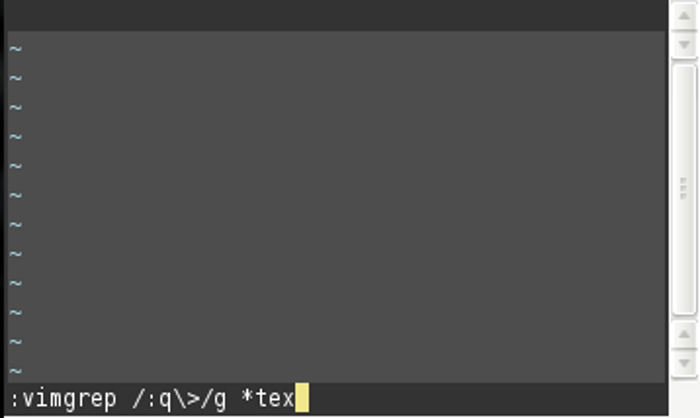
\includegraphics[width=0.7\textwidth]{sections/vimgrep/vimgrep1}
	\end{figure}
\end{frame}
\begin{frame}{:vimgrep}
	\begin{figure}[h!]
	  \caption{Resultado}
	  \centering
	    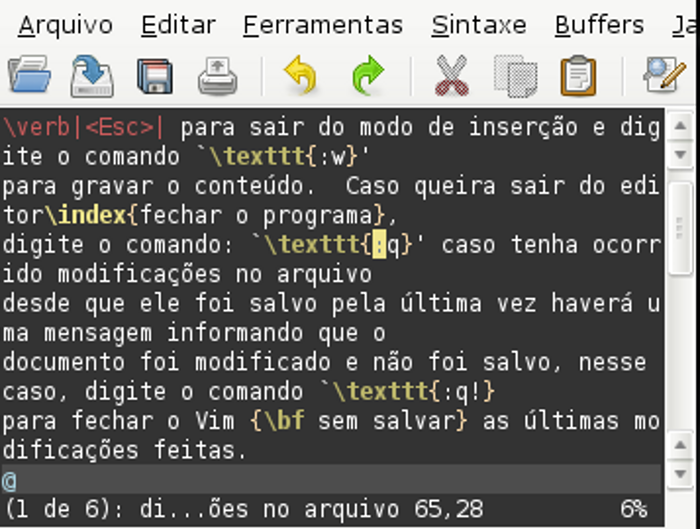
\includegraphics[width=0.7\textwidth]{sections/vimgrep/vimgrep2}
	\end{figure}
\end{frame}
\begin{frame}{:vimgrep}
	\begin{figure}[h!]
	  \caption{:copen}
	  \centering
	    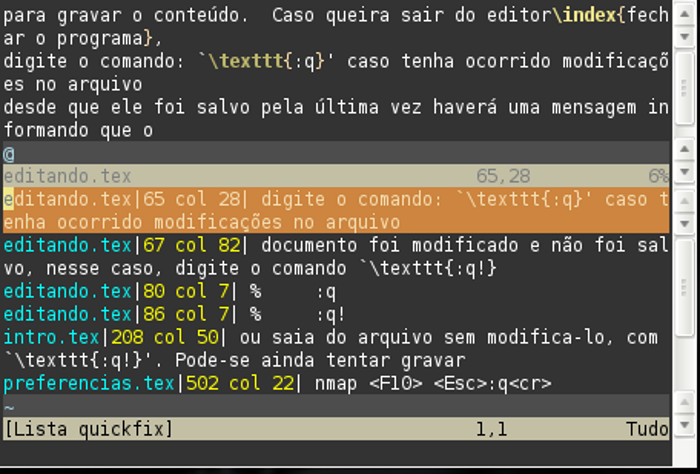
\includegraphics[width=0.7\textwidth]{sections/vimgrep/vimgrep3}
	\end{figure}
\end{frame}
\begin{frame}{:vimgrep}
	\begin{figure}[h!]
	  \caption{:cnext}
	  \centering
	    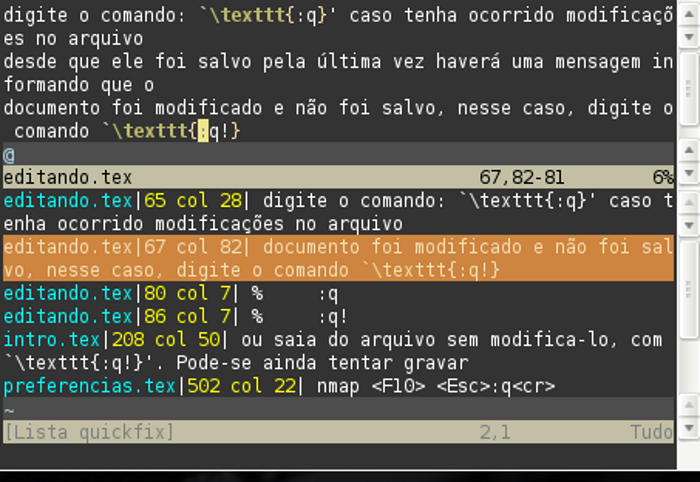
\includegraphics[width=0.7\textwidth]{sections/vimgrep/vimgrep4}
	\end{figure}
\end{frame}
